\section{可解码约束}
\label{sec:lossless-decodability}

码字各不相同，是不是就够了？看下面这张码表：
\[
 a\mapsto0,\qquad b\mapsto010,\qquad c\mapsto01,\qquad d\mapsto10 .
\]
四个码字互不相同，单独收到任何一个码字都能认出是哪个符号。可是收到拼接串$010$时，它既可以是$b$，也可以是$ca$（$01$接$0$），还可以是$ad$（$0$接$10$）。图~\ref{fig:lossless-ambiguous-parse}画出这三种切法。接收方没有分隔符，无法判断发送的是哪一条消息。

\begin{BookInlineFigure}
 \centering
 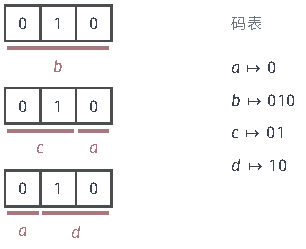
\includegraphics[width=52mm]{figures/07-probability/05-source-coding/tikz/lossless-ambiguous-parse/figure.pdf}
 \caption{码字互不相同、拼接后却有歧义的码。右侧为码表；同一个收到的串$010$（方框）有三种切分方式，红色横线下方是每段对应的符号，分别解读为$b$、$ca$和$ad$。}
 \label{fig:lossless-ambiguous-parse}
\end{BookInlineFigure}

所以要区分两层要求。码$c$称为\term{非奇异码}（nonsingular code），如果不同符号的码字不同，即$c$作为$\mathcal{X}\to\{0,1\}^{*}$的映射是单射。真正需要的是更强的一层：

\begin{definition}[唯一可译码]
\label{def:lossless-uniquely-decodable}
若码$c$的扩展~\eqref{eq:lossless-extension}在所有有限长符号序列上是单射，即对任意$m,n\geq1$与$x_{1:m}\in\mathcal{X}^m$、$y_{1:n}\in\mathcal{X}^n$，
\begin{equation}
 c(x_1)\cdots c(x_m)=c(y_1)\cdots c(y_n)\ \Longrightarrow\ m=n,\ x_{1:m}=y_{1:n},
 \label{eq:lossless-ud}
\end{equation}
则称$c$为\term{唯一可译码}（uniquely decodable code）。
\end{definition}

条件里$m$与$n$可以不同，这是为了把“同一个串能否被切成不同个数的码字”也排除掉。上面的例子中$010$一次切成一个码字、一次切成两个码字，所以那张码表非奇异却不唯一可译。唯一可译码中不能有空码字：若$c(x)$是空串，则$c(x)$与$c(xx)$相同，违反式~\eqref{eq:lossless-ud}。

唯一可译性只说“原则上能切开”，没说怎样切、要往后看多远。下面先看一类可以边读边切的码，再研究所有唯一可译码对码长的共同限制。

\subsection{前缀码}
\label{sec:lossless-prefix-codes}

开头例子的歧义来自一个码字是另一个码字的开头：$0$是$01$和$010$的开头，$01$又是$010$的开头。读到$0$时，解码器不知道这个码字是否已经结束。如果禁止这种情况，读到一个完整码字时就能立刻断开。

\begin{definition}[前缀码]
\label{def:lossless-prefix-code}
若串$s$可写成$s=ut$，则称$u$是$s$的前缀。若码$c$中没有一个码字是另一个码字的前缀，则称$c$为\term{前缀码}（prefix code），也称即时码。
\end{definition}

\paragraph{码树}
二进制串可以画在一棵二叉树上：从根出发，读到$0$走左支，读到$1$走右支，每个串对应一个结点，串长就是结点的深度。码字是树上的一些结点，从根到这些结点的路径合在一起称为\term{码树}（code tree）。“$u$是$s$的前缀”就是“结点$u$在根到结点$s$的路径上”。因此前缀码的码字恰好都是码树的叶结点：没有一个码字结点在另一个码字结点的下方。

图~\ref{fig:lossless-prefix-tree}(a)是贯穿例的码$0,10,110,111$。四个码字都是叶结点，所以它是前缀码。图中(b)是另一张码表$0,01,011,111$，码长同样是$1,2,3,3$，但$a$的码字$0$位于$b$的码字$01$上方，$01$又位于$011$上方，所以它不是前缀码。

\begin{BookInlineFigure}
 \centering
 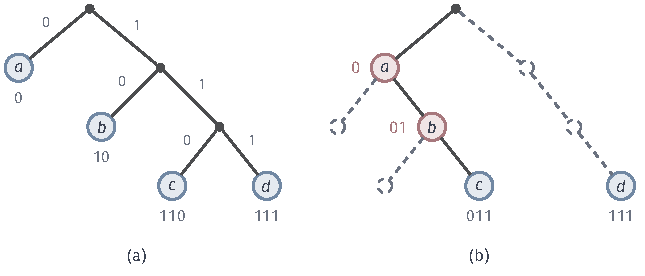
\includegraphics[width=110mm]{figures/07-probability/05-source-coding/tikz/lossless-prefix-tree/figure.pdf}
 \caption{码字作为二叉树的结点，左支读$0$、右支读$1$，结点下方或左侧是它的码字。(a)前缀码$0,10,110,111$，四个码字（蓝圈）都是叶结点。(b)码$0,01,011,111$，码长相同，但$a,b$的码字（红圈）位于其他码字的路径上；虚线和虚圈是路径经过的、不对应码字的结点。}
 \label{fig:lossless-prefix-tree}
\end{BookInlineFigure}

\paragraph{即时解码}
前缀码的解码过程是在码树上行走：从根出发，按收到的位逐步向下，到达叶结点就输出对应符号，然后回到根继续。到达叶结点时，这个码字一定已经结束，因为叶结点下面没有别的码字；而在到达叶结点之前，当前读到的串不是任何码字，也不可能提前断开。

用图~\ref{fig:lossless-prefix-tree}(a)解码$0100110$：读$0$到达叶$a$，输出$a$；读$1,0$到达叶$b$，输出$b$；读$0$输出$a$；读$1,1,0$到达叶$c$，输出$c$。每次输出都在读完该码字最后一位的那一刻完成，不需要看后面的位，这就是“即时”一词的含义。

\begin{theorem}[前缀码唯一可译]
\label{thm:lossless-prefix-ud}
前缀码是唯一可译码。
\end{theorem}

\begin{proof}
设$c(x_1)\cdots c(x_m)=c(y_1)\cdots c(y_n)$，记这个共同的串为$s$。$c(x_1)$与$c(y_1)$都是$s$的前缀，所以较短的一个是较长的一个的前缀。前缀码中这只能在两者相同时发生，于是$c(x_1)=c(y_1)$。前缀码中码字互不相同，所以$x_1=y_1$。

从$s$的两边去掉这个共同的码字，剩下的串仍满足同样的等式，对剩余部分重复上面的论证。每一步去掉同一个码字，直到某一边先用完。若$m<n$，左边用完时剩下的串是空串，右边却还有非空码字$c(y_{m+1})\cdots c(y_n)$；前缀码不含空码字，这不可能，因为空串是任何码字的前缀。所以$m=n$，且各位置的符号都相同。
\end{proof}

\paragraph{唯一可译但不是前缀码}
反过来不成立。图~\ref{fig:lossless-prefix-tree}(b)的码$a\mapsto0$、$b\mapsto01$、$c\mapsto011$、$d\mapsto111$不是前缀码，却是唯一可译码。把每个码字倒过来读，得到$0,10,110,111$，这正是(a)中的前缀码。收到整串后从右向左读，就是在倒序码的码树上即时解码，所以拼接串只有一种切法。

这张码的代价是解码延迟。设收到的串以$0$开头、后面跟着一串$1$。若串在$0111$处结束，它是$ad$；若是$01111$，它是$bd$；若是$011111$，它是$cd$；若是$0111111$，又回到$a$后接两个$d$。第一个码字是$0$、$01$还是$011$，取决于后面$1$的个数除以$3$的余数，解码器必须等这一串$1$全部结束才能确定第一个符号。前缀码没有这种等待，所以实际中几乎总用前缀码；下一小节说明，从码长的角度看，用前缀码也没有任何损失。

\subsection{Kraft–McMillan不等式}
\label{sec:lossless-kraft}

码长越短越好，但不能任意短：$\mathcal{X}$有四个符号，就不可能都用长度$1$的码字，因为长度为$1$的二进制串只有两个。一般地，码长受什么限制？下面先就前缀码回答，再把结论推广到全部唯一可译码。

\paragraph{码字占用的区间}
把码字$s=s_1s_2\cdots s_\ell$看成二进制小数$0.s_1s_2\cdots s_\ell$，它对应$[0,1)$中的区间
\[
 I(s)=\bigl[\,0.s_1\cdots s_\ell,\ 0.s_1\cdots s_\ell+2^{-\ell}\bigr),
\]
即所有以$s$开头的无限二进制展开所组成的数。区间的长度是$2^{-\ell}$：码字越短，占用的区间越长。在码树上，$I(s)$就是结点$s$下面整棵子树的“影子”。

两个码字$u,s$中若$u$是$s$的前缀，则$I(s)\subset I(u)$；若彼此都不是对方的前缀，则两者在某一位上第一次出现不同，一个在那一位取$0$、另一个取$1$，于是$I(u)$与$I(s)$不相交。所以前缀码的码字对应$[0,1)$中两两不交的区间。图~\ref{fig:lossless-kraft-intervals}第一行是贯穿例的码，四个区间恰好铺满$[0,1)$。

\begin{theorem}[Kraft不等式]
\label{thm:lossless-kraft}
设$\mathcal{X}=\{x_1,\dots,x_m\}$，正整数$\ell_1,\dots,\ell_m$。存在码长为$\ell_1,\dots,\ell_m$的二进制前缀码，当且仅当
\begin{equation}
 \sum_{i=1}^{m}2^{-\ell_i}\leq1 .
 \label{eq:lossless-kraft}
\end{equation}
\end{theorem}

\begin{proof}
必要性。前缀码的码字对应$[0,1)$中两两不交的区间，它们的长度之和不超过$[0,1)$的长度$1$，这就是式~\eqref{eq:lossless-kraft}。

充分性。把码长重新编号使$\ell_1\leq\ell_2\leq\cdots\leq\ell_m$，并令
\[
 F_1=0,\qquad F_i=\sum_{j<i}2^{-\ell_j}\quad(i=2,\dots,m).
\]
由式~\eqref{eq:lossless-kraft}，$F_i<1$。每个$2^{-\ell_j}$（$j<i$）都是$2^{-\ell_i}$的整数倍，所以$F_i$也是$2^{-\ell_i}$的整数倍，它的二进制展开在第$\ell_i$位之后全是$0$。取第$i$个码字为$F_i$二进制展开的前$\ell_i$位，于是
\[
 I(c(x_i))=\bigl[F_i,\,F_i+2^{-\ell_i}\bigr)=\bigl[F_i,\,F_{i+1}\bigr) ,
\]
这里$F_{m+1}=\sum_j2^{-\ell_j}\leq1$。这些区间首尾相接、两两不交。若某个码字$u$是另一个码字$s$的前缀，则$I(s)\subset I(u)$，与不交矛盾。所以得到的码是前缀码。
\end{proof}

充分性的证明给出了构造方法：码长从短到长排好，依次在$[0,1)$中从左往右截取长$2^{-\ell_i}$的区间。图~\ref{fig:lossless-kraft-intervals}第二行把这个方法用于码长$2,2,3,4$。依次得到
\[
 F_1=0,\quad F_2=\tfrac14,\quad F_3=\tfrac12,\quad F_4=\tfrac58 ,
\]
码字为$00,01,100,1010$。四个区间只占了$[0,1)$的$11/16$，剩下的$[11/16,1)$没有用上：这组码长满足Kraft不等式但不取等号，说明还有缩短码字的余地，例如把$1010$缩短为$101$仍是前缀码。

\begin{BookInlineFigure}
 \centering
 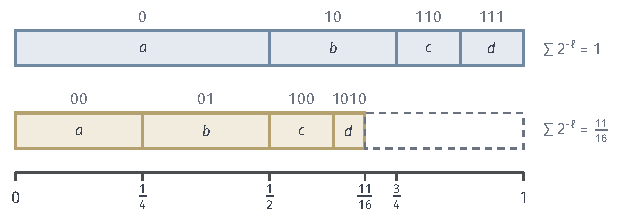
\includegraphics[width=106mm]{figures/07-probability/05-source-coding/tikz/lossless-kraft-intervals/figure.pdf}
 \caption{码字作为$[0,1)$中的二进区间，长度为$\ell$的码字占用长$2^{-\ell}$的区间，区间上方是码字。第一行（蓝）为码$0,10,110,111$，区间铺满$[0,1)$，Kraft和等于$1$。第二行（黄）为码长$2,2,3,4$按充分性证明构造的码$00,01,100,1010$，区间占去$11/16$，虚线框为未用的部分。}
 \label{fig:lossless-kraft-intervals}
\end{BookInlineFigure}

\paragraph{推广到唯一可译码}
唯一可译码的码字可以互为前缀，区间就可能嵌套，上面的必要性证明不再适用。可是码长仍然受同样的限制。McMillan的证明换了一个角度：不看单个码字，而是看把$k$个码字拼起来以后能得到多少种不同的串。

\begin{theorem}[McMillan不等式]
\label{thm:lossless-mcmillan}
任何二进制唯一可译码的码长都满足式~\eqref{eq:lossless-kraft}。
\end{theorem}

\begin{proof}
记$K=\sum_{x\in\mathcal{X}}2^{-\ell(x)}$，$\ell_{\max}=\max_x\ell(x)$。唯一可译码没有空码字，所以每个$\ell(x)\geq1$。固定正整数$k$，把$K$的$k$次方展开：
\[
 K^k=\sum_{x_1\in\mathcal{X}}\cdots\sum_{x_k\in\mathcal{X}}2^{-(\ell(x_1)+\cdots+\ell(x_k))}.
\]
求和的每一项对应一条长度为$k$的符号序列$x_{1:k}$，指数中的和正是它的码串$c(x_{1:k})$的长度。按码串长度$s$分组，记$N_s$为码串长度恰为$s$的序列个数，则
\[
 K^k=\sum_{s=k}^{k\ell_{\max}}N_s\,2^{-s}.
\]
唯一可译性说明不同的序列$x_{1:k}$给出不同的码串，而长度为$s$的二进制串只有$2^s$个，所以$N_s\leq2^s$。代入上式，每一项不超过$1$，项数为$k\ell_{\max}-k+1$，于是
\begin{equation}
 K^k\leq k(\ell_{\max}-1)+1 .
 \label{eq:lossless-mcmillan-count}
\end{equation}
若$K>1$，左边随$k$指数增长，右边只线性增长，$k$足够大时不等式必然被破坏。所以$K\leq1$。
\end{proof}

这个证明的直观是计数。若$K>1$，长序列的数目会比可用的二进制串增长得更快，迟早有两条序列不得不共用同一个码串。图~\ref{fig:lossless-mcmillan-growth}用码长$1,1,2$作例子，此时$K=1.25$。式~\eqref{eq:lossless-mcmillan-count}的右边为$k+1$，从$k=12$起$1.25^{k}$超过它。具体地，$1.25^{12}\approx14.55>13$：长度为$12$的符号序列给出的码串数目，已经超出了相应长度的二进制串所能容纳的数目，这三个码长不可能属于任何唯一可译码。

\begin{BookInlineFigure}
 \centering
 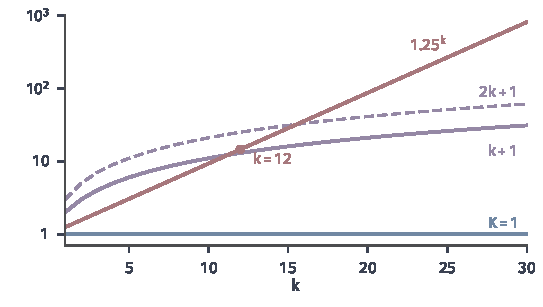
\includegraphics[width=92mm]{figures/07-probability/05-source-coding/matplotlib/lossless-mcmillan-growth/figure.pdf}
 \caption{McMillan计数论证，纵轴为对数坐标。红线为码长$1,1,2$的$K^k=1.25^k$，紫色实线为$\ell_{\max}=2$时的上界$k+1$，二者在红点$k=12$处交叉；紫色虚线为$\ell_{\max}=3$时的上界$2k+1$。蓝线为满足等号的码长$1,2,3,3$，$K^k=1$始终在上界之下。}
 \label{fig:lossless-mcmillan-growth}
\end{BookInlineFigure}

定理~\ref{thm:lossless-kraft}与定理~\ref{thm:lossless-mcmillan}合起来称为\term{Kraft–McMillan不等式}（Kraft–McMillan inequality）：任何唯一可译码的码长满足式~\eqref{eq:lossless-kraft}，而满足式~\eqref{eq:lossless-kraft}的码长都能由前缀码实现。因此，凡是只依赖码长的指标，例如平均码长，在唯一可译码中能达到的值，用前缀码都能达到。前面那张倒序的唯一可译码$0,01,011,111$没有带来任何码长上的好处，只多了解码延迟。

\paragraph{充分性说的是码长}
定理~\ref{thm:lossless-kraft}的充分性只保证“存在”一个具有这些码长的前缀码，并不说任何一种具有这些码长的码字分配都可以唯一解码。码长$1,2,2$满足
\[
 2^{-1}+2^{-2}+2^{-2}=1 ,
\]
按构造得到前缀码$0,10,11$。若随手把码字取成$0,00,11$，码长相同，但$00$既可以是第二个符号，也可以是第一个符号出现两次，不唯一可译。码长合格之后，码字仍要按证明中的方法（或其他保证前缀性的方法）来分配。
